
\article{Технологии}{Готовим травильный аквариум}{

\subarticle{Введение}

\noindent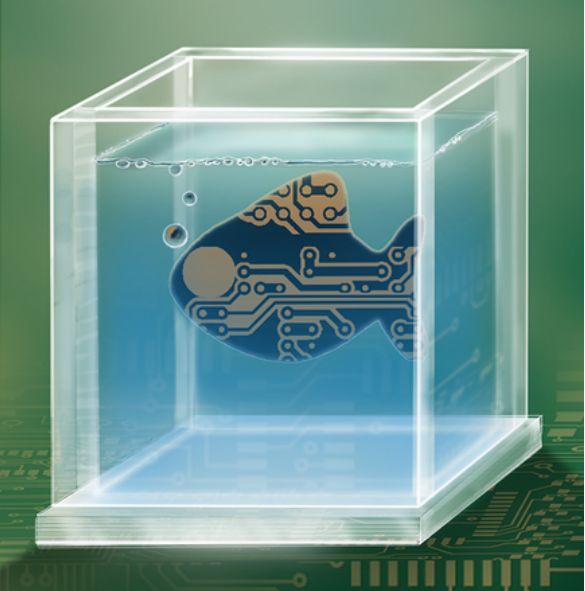
\includegraphics[width=0.3\textwidth]{00/fig/smit/ee000008.png}

Данная разработка, как и любая другая у меня, делалась по принципу увидел клевую
вещь\ --- захотел такую же. Сей проект\ --- это творчески доработанный аквариум
для травления печатных плат в домашних условиях. Этих аквариумов уже гуляет
солидное количество по сети.

Я хоть травлю платы не слишком часто, но иногда случается и так получается, что
эти самые платы у меня плохо получаются. \smiley\ И вот однажды в поисках
секрета получения хороших плат я наткнулся на
\href{http://we.easyelectronics.ru/Tools/akvarium-dlya-travleniya-pechatnyh-plat.html}{вот
эту штуку}.

Мне она понравилась и я захотел такую же. Но как и любая идея которая у меня
зреет, эта ждала своего часа довольно долго. Пока в один прекрасный день я не
уволился с работы, а до устройства на следующую у меня оставались три недели
лишнего отпуска. Их-то я и решил потратить с пользой. Что из этого получилось я
и хочу вам показать.

\subarticle{Выбор концепции и комплектующих или начинаем готовку}

Итак задача ясна и я начал думать как её осуществить. Тупо повторить разработку
\textbf{JeckDigger}\ (ссылка выше) мне было неинтересно, ведь впереди целых три
недели! И я начал думать, что же такого интересного можно сделать.
С самим аквариум из оргстекла все ясно, тут что-то новое придумать сложно.
Единственное, если у JeckDigger аквариум изготавливался из подручных средств, то
у меня был доступ к фрезерному станку и я решил им воспользоваться по полной.
Быстро наваял чертежи аквариума и мне их по дружбе сфрезировали. В качестве
материала я использовал оргстекло толщиной 5 мм. Получилось как-то так :

\noindent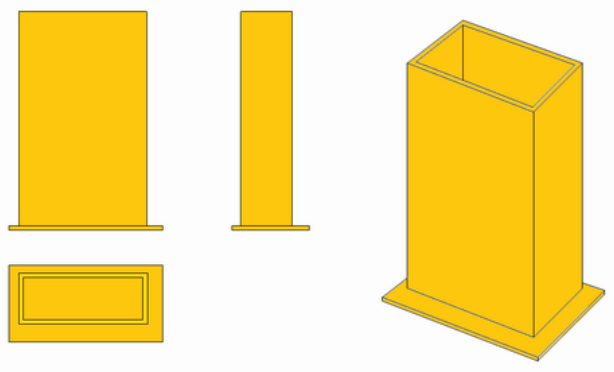
\includegraphics[width=\textwidth]{00/fig/smit/ee000017.png}
\textbf{Чертеж аквариума}

\href{}{Файлы чертежей в формате .dwg}

А вот и деталировка:

\noindent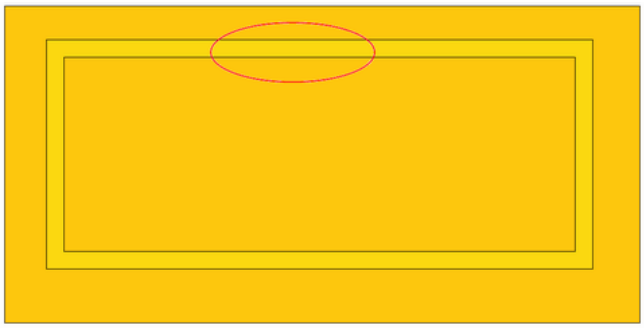
\includegraphics[width=\textwidth]{00/fig/smit/ee000018.png}
\textbf{Основание}

% Красным выделено углубление 2\,мм. Которое играет роль своеобразных
% направляющих. В них устанавливаются стенки аквариума. Сделал я их для лучшего
% позиционирования при слеивании аквариума ибо придавливать вертикальную стенку
% авквариума смазанную клеем к гладкой плоскости основание то еще удовольствие,
% добиться параллельности всех стенок очень сложно. А в таком варианте все удобно
% становится, да и клей в углубление хорошо заливается и не размазывается по всей
% поверхности.
% 
% \noindent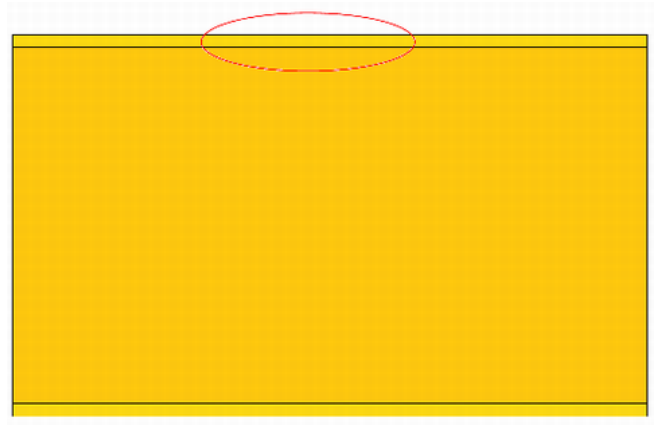
\includegraphics[width=\columnwidth]{fig/00/smit/ee000019.png}
% \texbf{Фронтальная стенка}
% 
% Красным выделено углубление 2\,мм в виде ступеньки. Сделано оно опять же для
% удобства склеивания и для того, чтобы на выходе получить аккуратный
% параллелепипед аквариума. \smiley
% 
% \noindent
\includegraphics[width=\columnwidth]{fig/00/smit/ee000020.png}
% \texbf{Боковая стенка}
% 
% Здесь никаких извращений. Обычный прямоугольник. \smiley
% \bigskip
% 
% Итак с самим аквариумом разобрались. Но этого конечно же мало для полного
% счастья. Как и у JeckDigger я решил добавить туда стандартный аквариумный
% распылитель.
% 
% \noindent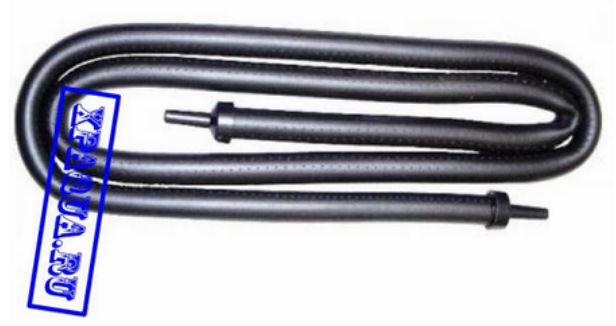
\includegraphics[width=\columnwidth]{fig/00/smit/ee000021.png}
% \texbf{Аквариумный распылитель}
% 
% Распылитель служит своеобразной <<палкой-мешалкой>> травящего
% раствора. Ходит слух, что это помогает ускорить процесс травления. Скажу
% честно, я без понятия правда это или нет, но идея мне понравилась.
% 
% Для распылителя был необходим компрессор. Я выбрал самый
% миниатюрный какой только нашел\ --- АС-500.
% 
% \noindent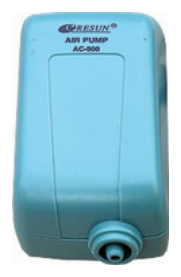
\includegraphics[width=0.5\columnwidth]{fig/00/smit/ee000022.png}
% \texbf{Аквариумный компрессор}
% 
% Объем нашего аквариума небольшой поэтому такого компрессора вполне хватит.
% 
% Но если вы думаете, что это все, то вы плохо меня знаете. \smiley\ Разойдясь я
% уже не мог остановиться. Я решил прикрутить к всему этому добру нагреватель с
% температурной регулировкой. Опять же ходит слух, что в теплой воде процесс
% травления идет быстрее\footnote{\ а если объединить компрессор и нагреватель, то
% плата должна травиться вообще в две секунды \smiley\ }. Сказано\ --- сделано. С
% качестве нагревателя был использован обычный аквариумный нагреватель мощностью
% 75 Вт.
% 
% \noindent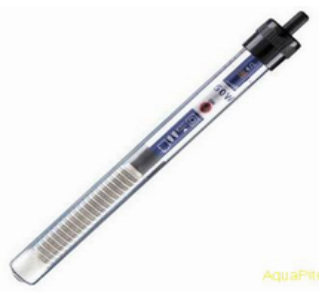
\includegraphics[width=\columnwidth]{fig/00/smit/ee000023.png}
% \texbf{Аквариумный нагреватель}
% 
% \emph{Примечание 2\ --- Не обращайте внимания, что на картинке указанна
% мощность 50\,Вт. Просто достойной фотографии нагревателя, который
% приобрел я сделать не удалось, поэтому в срочном порядке был подключен
% Google \smiley}.
% 
% Правда нагреватель пришлось доработать, но об этом речь пойдет дальше.
% 
% Итак, нагреватель есть, осталось прикрутить к нему терморегулятор. И тут
% появилась дилема: либо собирать схему самому либо купить уже готовый.
% После непродолжительных дебатов с самим собой решение было принято в пользу
% покупного. Ибо, делать плату самому было лень. Да и как её сделаешь, если
% аквариум для травления еще не готов? \smiley\ Налицо парадокс. \smiley
% 
% Свободного времени было хоть отбавляй, поэтому не откладывая дело в долгий ящик
% я пошел на радио рынок. После непродолжительных поисков я нашел, что искал:
% 
% \noindent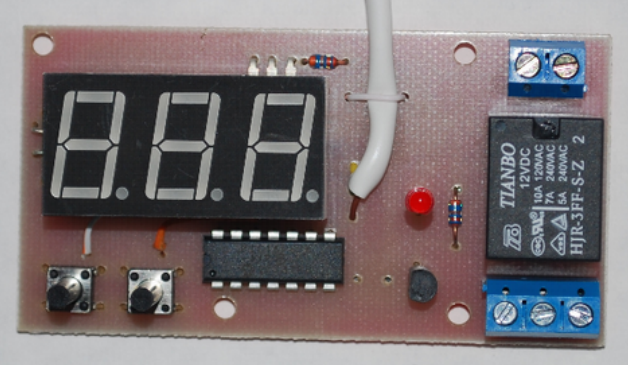
\includegraphics[width=\columnwidth]{fig/00/smit/ee000024.png}
% \texbf{Плата регулятора температуры}
% 
% По параметром он конечно немного превосходил мои скромные запросы, но я был не в
% обиде.
% 
% Итак, вроде с большего было понятно что делать, оставалось обдумать детали.
% 
% Например, я захотел не только регулировать температуру кнопками, но и
% включать/выключать распылитель при помощи кнопки. Так же появилась небольшая
% проблема связанная с питанием. Заключалась она в том, что нагреватель и
% компрессор работают от напряжения $\sim$220\,В, плюс для питания остальной
% электроники планировалось использовать зарядное устройство для сотового
% телефона, а оно так же подключалось в сети $\sim$220\,В. А это означало, что для
% работы аквариума необходимо было занимать аж три розетки, что меня нисколько не
% устраивало. Поэтому я решил сделать, так чтобы для питания прибора можно было
% обойтись одним сетевым кабелем. Так же я решил всю электронику, включая
% компрессор запихнуть в деревянное основание, на которое уже устанавливать сам
% аквариум из оргстекла. Что же, концепция, с большего была ясна\ --- осталось
% дело за малым. \smiley

}{}
%Алекс Смит {\href{mailto:zamuhrishka\@inbox.ru}}
